% ---------------------------------------------------------------------- %

\documentclass[letterpaper,10pt]{article}



\pagestyle{empty}

\usepackage[table]{xcolor}
\usepackage{color, colortbl}
\usepackage{tabularx}
\usepackage{amssymb}
\usepackage{enumerate}

\definecolor{LightGray}{gray}{0.9}

\usepackage{amsmath}
\usepackage{amscd}
\usepackage{url}

\usepackage{graphicx}


\title{Installing AIMBAT}
\author{Seismo Group}
\date{\today}

\begin{document}
\maketitle

% ************************************************************* %
%                                                               %
%                       MACPORT UPGRADES                        %
%                                                               %
% ************************************************************* %

\section{Macport Problems}

You may run into problems with AIMBAT if your Macport version is not compatible with your operating system version. For example, if you used Macports for OS X 10.8 to install AIMBAT, then upgraded your operating system ot OS X 10.9, you may find that AIMBAT no longer works properly. You will need to upgrade Macports to fix this error.

Do not uninstall MacPorts unless you know what you are doing, uninstalling MacPorts may get rid of other programs you installed using MacPorts. However, if you are sure you want to do so, see here for instructions: \url{https://guide.macports.org/chunked/installing.macports.uninstalling.html}. 

% \begin{figure}[h!]
%   \centering
%   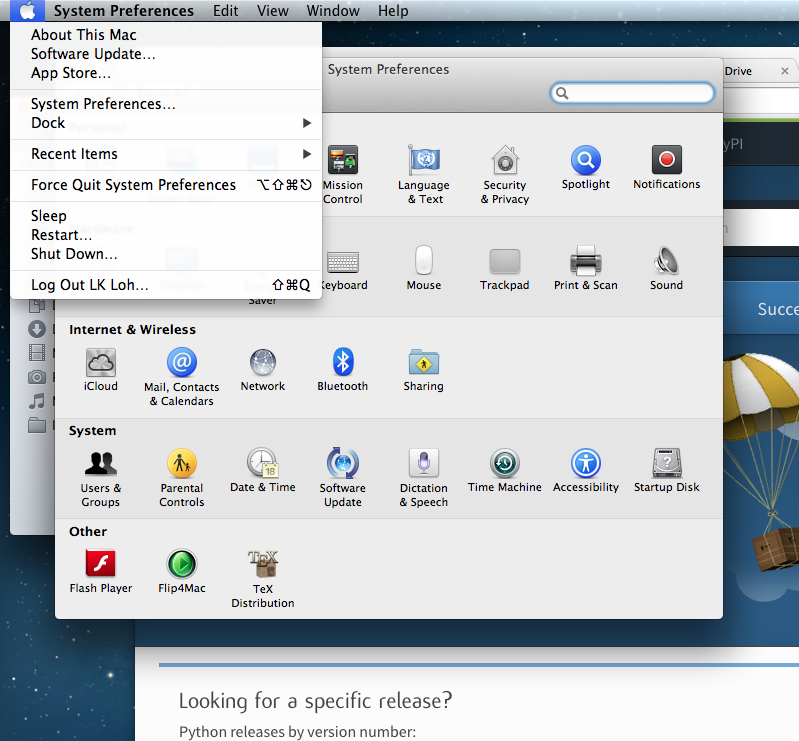
\includegraphics[width=0.5\textwidth]{images/system_preferences}
%   \caption{Console}
%   \label{fig:system_preferences}
% \end{figure}


% ************************************************************* %
%                                                               %
%                       MACPORT UPGRADES                        %
%                                                               %
% ************************************************************* %

% ************************************************************* %
%                                                               %
%                      PIP INSTALLATION                         %
%                                                               %
% ************************************************************* %

\section{Installing Python with Pip}

Be careful with the operating system. For OS X 10.9 and above, Python 2.7 is not fully compatible and there may be problems installing python with Pip. Best to use Enthought Canopy or Python 3 with OS X 10.9. 

% ************************************************************* %
%                                                               %
%                      PIP INSTALLATION                         %
%                                                               %
% ************************************************************* %

% ************************************************************* %
%                                                               %
%                     SETTING THE PYTHON PATH                   %
%                                                               %
% ************************************************************* %

\section{Setting the Python Path to the scripts}

You are asked to add the path to the AIMBAT scripts in your file. To do that, you add them to the \verb".bashrc" file. There are other files you could add it to that work as well, such as the \verb".profile" or \verb".bash_profile" files. You can see the files by opening the terminal and doing \verb"ls -a" to see all the hidden files, and open then by doing \verb"vi .bashrc" in vim, for instance.

To ensure you can open a script, you need to add
\begin{verbatim}
  export PATH=$PATH:<path-to-folder-with-scripts>
  export PYTHONPATH=$PYTHONPATH:<path-to-folder-with-scripts>
\end{verbatim}
to the \verb".bashrc" file. We recommend adding the paths to the \verb".bashrc" file, for reasons listed here: \url{http://stackoverflow.com/questions/415403/whats-the-difference-between-bashrc-bash-profile-and-environment}.


% ************************************************************* %
%                                                               %
%                     SETTING THE PYTHON PATH                   %
%                                                               %
% ************************************************************* %

% ************************************************************* %
%                                                               %
%                   TERMINAL COMMANDS STOP WORKING              %
%                                                               %
% ************************************************************* %

\section{Terminal Commands stop working}

If ever the terminal commands such as \verb"ls" stop working in the terminal, it could be that something went wrong with a path in the \verb".bashrc" or \verb".profile" files. If that happens you may not be able to open them in vim as that command would have stopped working as well. Instead, in the terminal, you do

\begin{verbatim}
  PATH=/bin:${PATH}
  PATH=/usr/bin:${PATH}
\end{verbatim}

And that should allow the commands to start working again. Figure out what you did wrong and remove that command. 

% ************************************************************* %
%                                                               %
%                   TERMINAL COMMANDS STOP WORKING              %
%                                                               %
% ************************************************************* %

% ************************************************************* %
%                                                               %
%                    INSTALLING ENTHOUGHT CANOPY                %
%                                                               %
% ************************************************************* %

\section{Installing Enthought Canopy}

Occasionally, Enthought Canopy may not open the default setup environment after you downloaded and tried to install it. If this happens, open the Canopy package, go to ``Preferences'', and select Canopy as your default environment. 


\begin{figure}[h!]
  \centering
  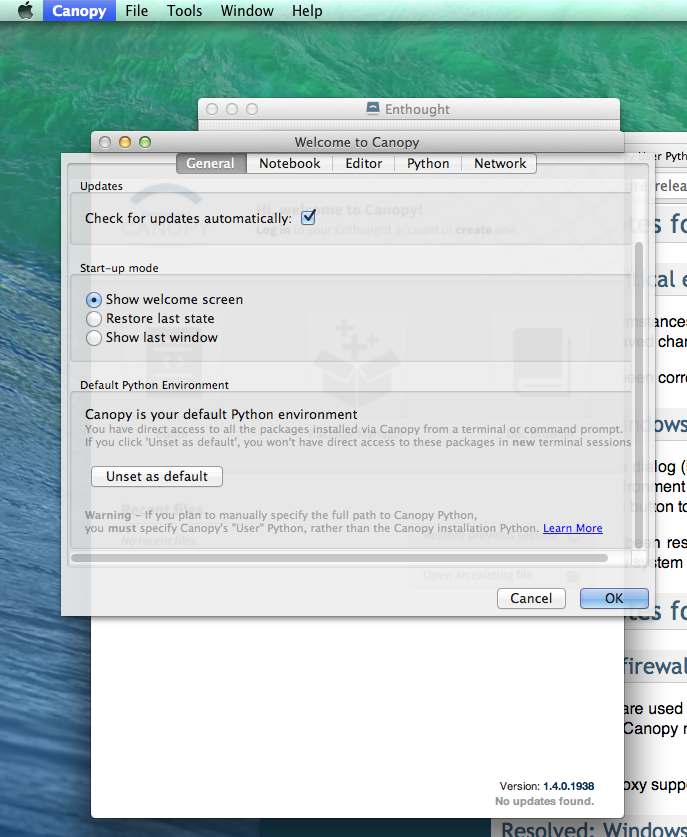
\includegraphics[width=0.5\textwidth]{images/enthought_as_default}
  \caption{Manually opening the default setup environment}
  \label{fig:enthought_as_default}
\end{figure}

% ************************************************************* %
%                                                               %
%                    INSTALLING ENTHOUGHT CANOPY                %
%                                                               %
% ************************************************************* %

% ************************************************************* %
%                                                               %
%                  UNINSTALLING ENTHOUGHT CANOPY                %
%                                                               %
% ************************************************************* %

\section{Uninstalling Enthought Canopy}

The official Enthought gives suggestions on uninstalling here: \url{https://support.enthought.com/entries/23580651-Uninstalling-Canopy}

STEP 1: From the Canopy preferences menu, unset Canopy as your default Python.

\begin{figure}[h!]
  \centering
  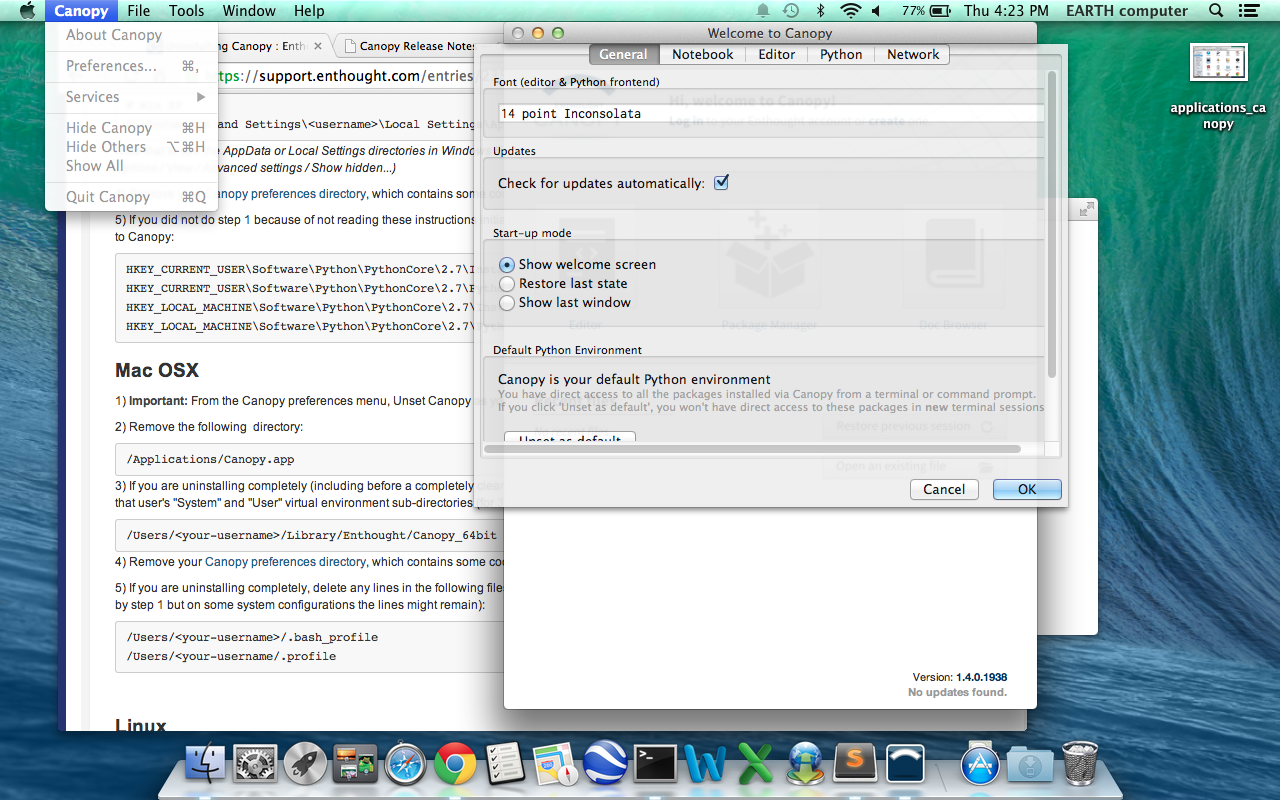
\includegraphics[width=0.5\textwidth]{images/canopy_preferences}
  \caption{Canopy preferences}
  \label{fig:canopy_preferences}
\end{figure}

STEP 2: for each Canopy user, delete the following directory which contains that user's ``System'' and ``User'' virtual environment subdirections.

STEP 3: Delete Canopy from the Applications folder. 

\begin{figure}[h!]
  \centering
  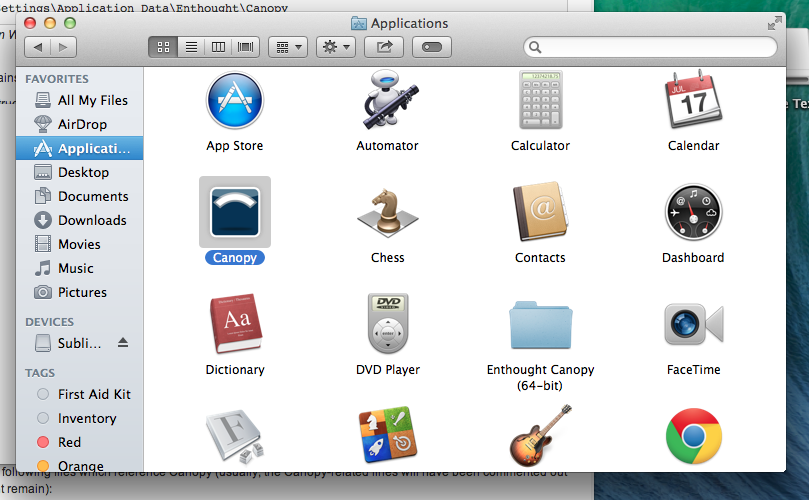
\includegraphics[width=0.5\textwidth]{images/applications_canopy}
  \caption{applications canopy}
  \label{fig:applications_canopy}
\end{figure}

STEP 4: Clean up the hidden files. Delete anything referencing Canopy or Enthought in the hidden files, as evidence by referencing \verb"ls -a" in your home directory. Check the \verb".bashrc" and \verb".profile" directories first. If Enthought is not completely gone, this happens if you call Python:

\begin{figure}[h!]
  \centering
  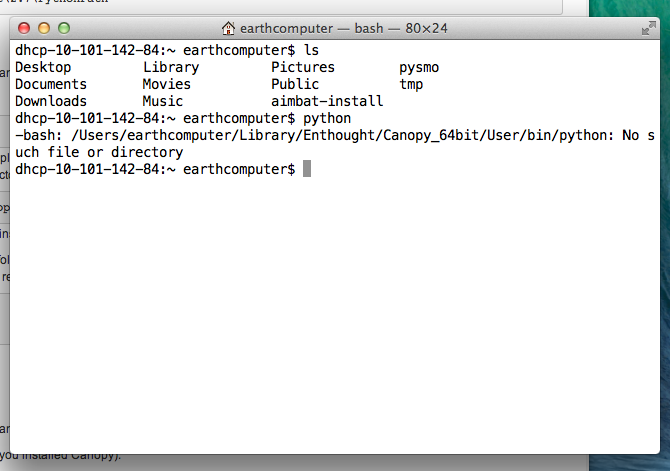
\includegraphics[width=0.5\textwidth]{images/residue}
  \caption{Residue}
  \label{fig:residue}
\end{figure}

STEP 5: (Optional). Keep doing \texttt{which python} and cleaning the python files that show up, until \texttt{which python} gives you nothing when you type it in the terminal. 


% ************************************************************* %
%                                                               %
%                  UNINSTALLING ENTHOUGHT CANOPY                %
%                                                               %
% ************************************************************* %

% ************************************************************* %
%                                                               %
%                  PATH TO FILES NOT FOUND                      %
%                                                               %
% ************************************************************* %

\section{Path to python files not found}


After adding the path to your directory with scripts in \verb".bashrc", you still need to source the \verb".bashrc" files in \verb".profile", or the system may not find the directory. 

This explanation from \url{http://publib.boulder.ibm.com/infocenter/pseries/v5r3/index.jsp?topic=/com.ibm.aix.baseadmn/doc/baseadmndita/prof_file.htm} explains how the profile file is sourced. Note that this one will override the file in \texttt{/etc/profile}.

\begin{figure}[h!]
  \centering
  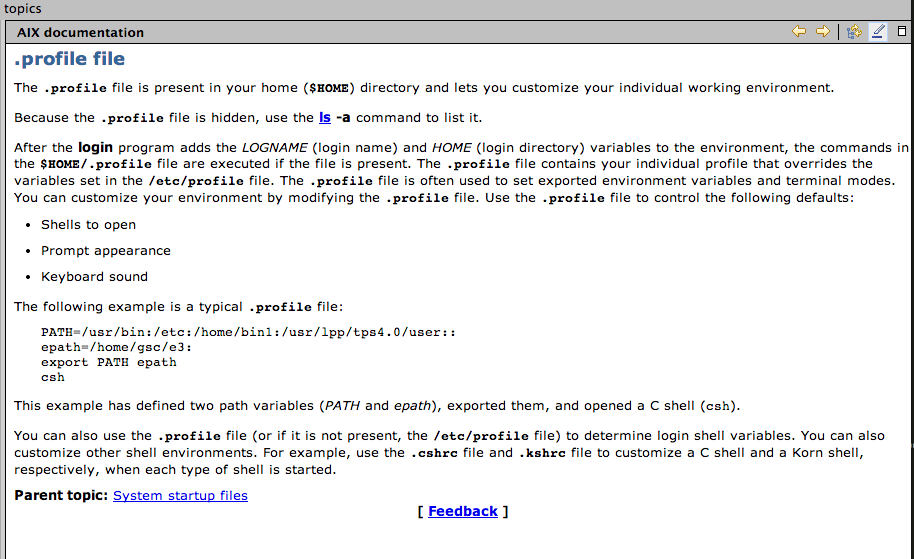
\includegraphics[width=0.5\textwidth]{images/profile_file}
  \caption{Profile file}
  \label{fig:profile_file}
\end{figure}

This explanation from \url{http://linux.die.net/man/1/bash} explains how the bashrc file is sourced. 

\begin{figure}[h!]
  \centering
  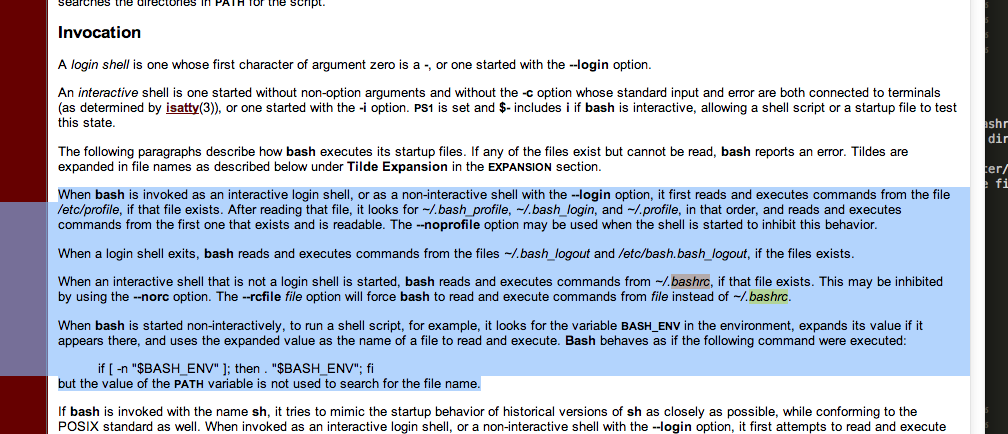
\includegraphics[width=0.5\textwidth]{images/bashrc_file}
  \caption{Bashrc file}
  \label{fig:bashrc_file}
\end{figure}

This is what the bashrc and profile files should look like on your home directory:

\begin{figure}[h!]
  \centering
  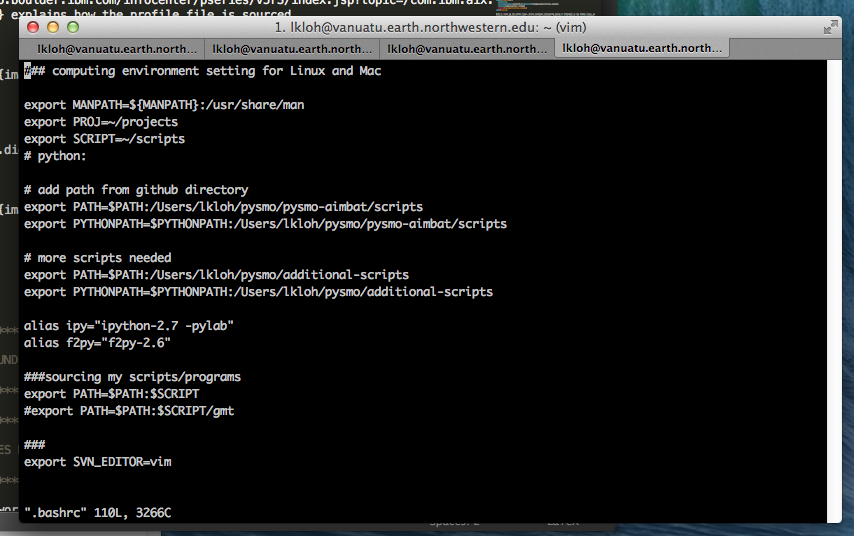
\includegraphics[width=0.5\textwidth]{images/bashrc_home}
  \caption{Bashrc home}
  \label{fig:bashrc_home}
\end{figure}

\begin{figure}[h!]
  \centering
  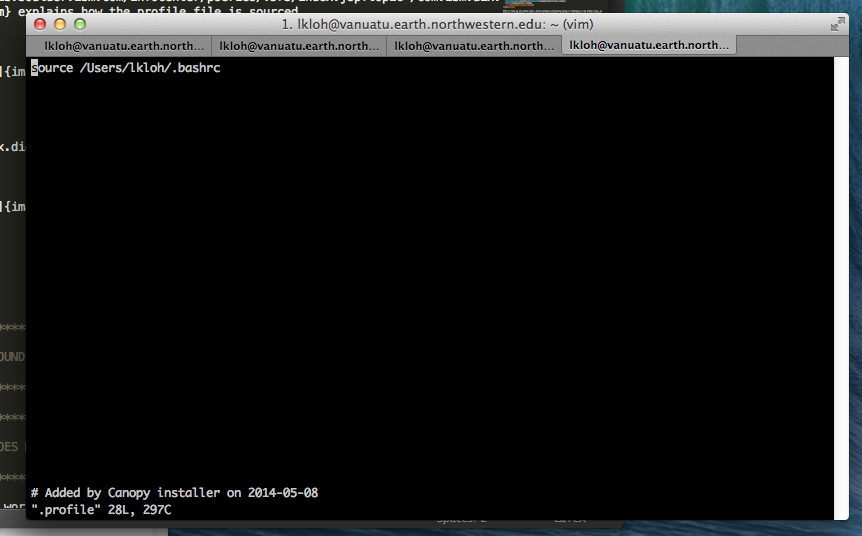
\includegraphics[width=0.5\textwidth]{images/profile_home}
  \caption{Profile home}
  \label{fig:profile_home}
\end{figure}


% ************************************************************* %
%                                                               %
%                  PATH TO FILES NOT FOUND                      %
%                                                               %
% ************************************************************* %

% ************************************************************* %
%                                                               %
%               PICKING TRAVEL TIMES DOES NOT WORK              %
%                                                               %
% ************************************************************* %

\section{Picking Travel Times does not work}

If you run \verb"ttick.py <Event name>.bhz.pkl", a GUI will pop up for you to manually pick the travel times by pressing the keyboard. If typing on the keyboard as directed does not allow you to pick travel times, it could be a problem with the keyboard settings, or the matplotlib backend. 

To fix this, first look for the \verb".matplotlib" directory. It is hidden so in your home directory do \verb"ls -a" to find it.

\begin{figure}[h!]
  \centering
  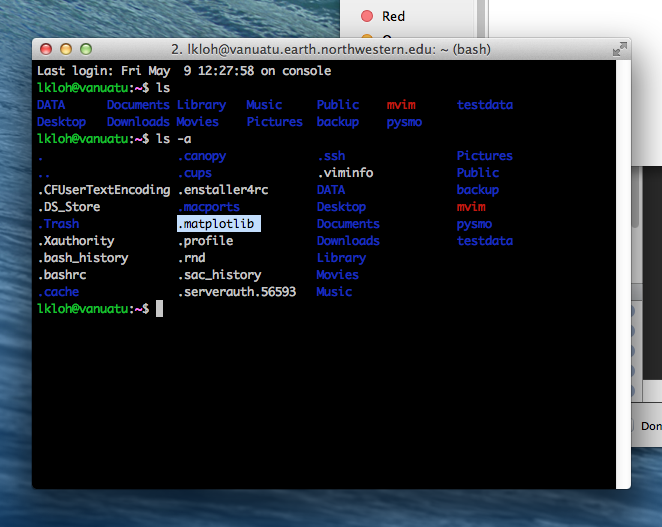
\includegraphics[width=0.5\textwidth]{images/matplotlib_hidden_directory}
  \caption{Matplotlib hidden directory}
  \label{fig:matplotlib_hidden_directory}
\end{figure}

Once you have found the \verb".matplotlib" directory, cd into it, and then look for the \verb"matplotlibrc" file. 

\begin{figure}[h!]
  \centering
  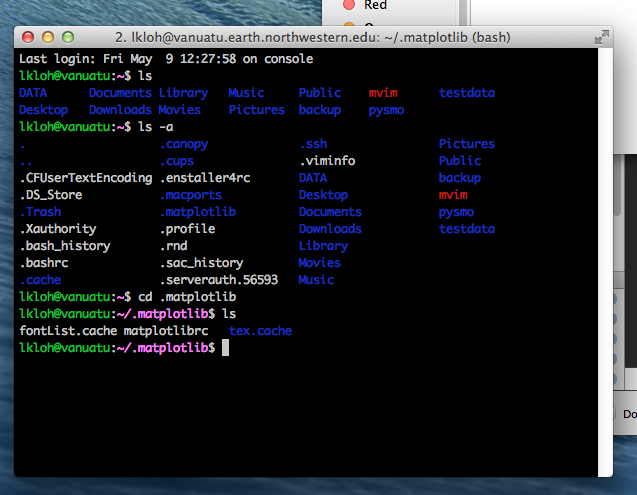
\includegraphics[width=0.5\textwidth]{images/files_in_matplotlib}
  \caption{.matplotlib files within}
  \label{fig:files_in_matplotlib}
\end{figure}

Inside that file, ensure the backend is set to:

\begin{verbatim}
  backend : TkAgg
\end{verbatim}

Comment out the other backends! 

\begin{figure}[h!]
  \centering
  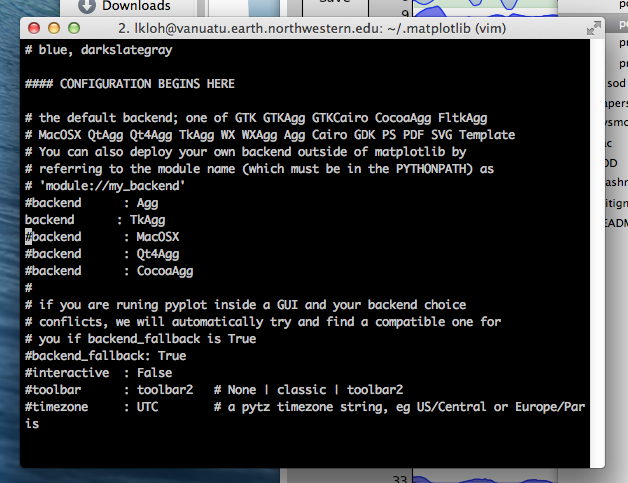
\includegraphics[width=0.5\textwidth]{images/matplotlibrc_file}
  \caption{Matplotlibrc backend}
  \label{fig:matplotlibrc_file}
\end{figure}

% ************************************************************* %
%                                                               %
%               PICKING TRAVEL TIMES DOES NOT WORK              %
%                                                               %
% ************************************************************* %

% ************************************************************* %
%                                                               %
%                   PROBLEMS WITH FINDING TRAVEL TIMES          %
%                                                               %
% ************************************************************* %

\section{Travel Times}

If one of the seismograms being picked does not fit completely within the green (computer) window, nad you hit \framebox[1.1\width]{ICCC-A} or \framebox[1.1\width]{MCCC}, you will get an error message complaining about the exact seismogram which is too short. Deselect it. 

\begin{figure}[h!]
  \centering
  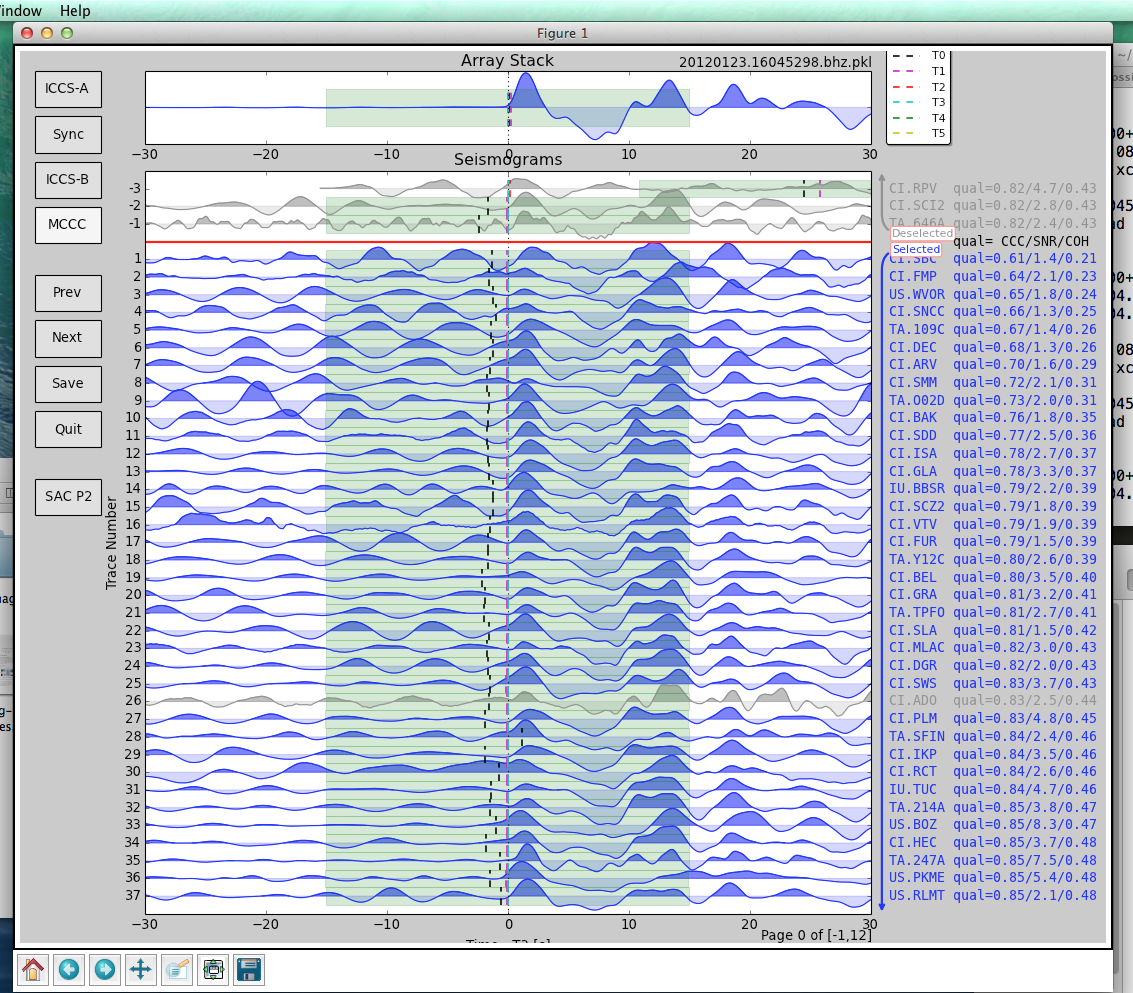
\includegraphics[width=0.5\textwidth]{images/not_enough_sample}
  \caption{Sample not within computated (green) region}
  \label{fig:not_enough_sample}
\end{figure}



% ************************************************************* %
%                                                               %
%                   PROBLEMS WITH TRAVEL TIMES                  %
%                                                               %
% ************************************************************* %

% ------------------------------------------------------------------------- %

\end{document}

% --------------------------------- END --------------------------------- %
